\documentclass[12pt]{article}

\newcommand{\reporttitle}{Crouzeix-Raviart Element for the Stokes Problem}
\newcommand{\accentcolor}{solarized-red}
\newcommand{\urlcolor}{solarized-yellow}

\usepackage{amsmath}
\usepackage{mathrsfs}
\usepackage{amsthm}
\usepackage{amsfonts}
\usepackage{bm}
\usepackage{amssymb}
\usepackage{stmaryrd}

% Sets.
\newcommand{\R}{\mathbb{R}}
\newcommand{\RT}{\mathbb{R}^2}
\newcommand{\N}{\mathbb{N}}

\newcommand{\PK}[1]{\mathbb{P}_{#1}}

\newcommand{\LT}{\mathscr{L}^2}
\newcommand{\HO}{\mathscr{H}^1}
\newcommand{\Tau}{\mathcal{T}}

% Vectors and operators.
\newcommand{\Vector}[1]{\bm{#1}}
\newcommand{\Operator}[1]{\textcolor{solarized-green}{#1}}

% Matrices.
\newcommand{\MA}{\mathcal{A}}
\newcommand{\MB}{\mathcal{B}}
\newcommand{\VF}{\mathcal{F}}

% Gradient and divergence.
\newcommand{\grad}{\Vector{\nabla}}
\newcommand{\diver}{\text{div }}

% Span.
\newcommand{\Span}[1]{\text{span} \left\{ #1 \right\}}

% Bilinear operators.
\newcommand{\boa}[2]{\Operator{a}(#1, #2)}
\newcommand{\bob}[2]{\Operator{b}(#1, #2)}

% Fortin.
\newcommand{\tfortin}{\Operator{\tilde{\Pi}}}
\newcommand{\fortin}{\Operator{\Pi}}
\newcommand{\fortinptpz}{\Operator{\Pi^2_0}}

% Redefinition.
\newcommand{\Exists}{\exists ~}
\newcommand{\Forall}{\forall ~}

% Theorems.
\newtheorem{theorem}{Theorem}[section]
\newtheorem{lemma}{Lemma}[section]
\newtheorem{proposition}{Proposition}[section]

\newtheorem*{theorem*}{Theorem}

\usepackage{courier}
\usepackage{listings}

\lstdefinestyle{default}{
	basicstyle=\ttfamily\color{solarized-base01},
	breakatwhitespace=false,
	breaklines=true,
	keepspaces=true,
	showspaces=false,
	showstringspaces=false,
	showtabs=false,
	tabsize=2
}

% MATLAB, if needed.

% \lstdefinestyle{matlab}{
% 	commentstyle=\color{solarized-green},
% 	keywordstyle=\color{solarized-blue},
% 	stringstyle=\color{solarized-orange},
% 	basicstyle=\ttfamily\color{solarized-base01},
% 	breakatwhitespace=false,
% 	breaklines=true,
% 	captionpos=b,
% 	keepspaces=true,
% 	showspaces=false,
% 	language=matlab,
% 	showstringspaces=false,
% 	showtabs=false,
% 	tabsize=4
% }

\lstset{style=default}

\usepackage{nameref}
\usepackage{multicol}
\usepackage{titlesec}

\usepackage{enumerate}

\usepackage{graphicx}
\graphicspath{{../gallery/}}

\usepackage{xcolor-solarized}
\color{solarized-base02}

\usepackage[T1]{fontenc}
\usepackage[utf8]{inputenc}

\usepackage[a4paper]{geometry}
\geometry{
	inner=20mm,
	outer=20mm,
	top=30mm,
	bottom=30mm,
	heightrounded,
	marginparwidth=50pt,
	marginparsep=20pt,
	headsep=25pt,
	headheight=30pt
}

\usepackage{hyperref}
\hypersetup{
	linktocpage=true,
	colorlinks=true,
	linkcolor=\accentcolor,
	urlcolor=\urlcolor,
	pdftitle={\reporttitle},
	pdfpagemode=FullScreen,
	pdfauthor={Andrea Di Antonio}
}

\usepackage{fancyhdr}
\pagestyle{fancy}
\fancyhf{}
\fancyhead[R]{Andrea Di Antonio}
\fancyhead[L]{\reporttitle}
\fancyfoot[C]{\thepage}

\title{\reporttitle}
\author{Andrea Di Antonio, 858798 \\ \hyperlink{mailto:a.diantonio1@campus.unimib.it}{a.diantonio1@campus.unimib.it}}
\date{Exam session of February 29, 2024 \\ Academic Year 2023-24}

\setcounter{tocdepth}{2}

\begin{document}
	\pagenumbering{roman}
	\maketitle
	\thispagestyle{fancy}

	\begin{abstract}
		\begin{center}
			Report for the course \textit{Metodi Numerici Avanzati per Equazioni alle Derivate Parziali} focusing on the definition, implementation\footnote{Written in MATLAB.}, and convergence analysis of the Crouzeix-Raviart element for the Stokes Problem.
		\end{center}
	\end{abstract}

	\newpage
	\tableofcontents

	\newpage
	\pagenumbering{arabic}
	\section{Formulations of the Stokes Problem}
	Consider the domain $\Omega = [0, 1] \times [0, 1] \subset \mathbb{R}^2$. The aim is to find $\Vector{u} \in \left[ C^2(\Omega) \right]^2$ and $p \in C^1(\Omega)$ such that, for any $\Vector{f} \in \left[ C(\Omega) \right]^2$, the following equations hold:

\begin{gather}
    \begin{cases} \label{strong_stokes}
        - \Delta \Vector{u} - \grad p = \Vector{f} & \Forall \Vector{x} \in \Omega, \\
        \diver \Vector{u} = 0 & \Forall \Vector{x} \in \Omega, \\
        \Vector{u} = 0 & \Forall \Vector{x} \in \partial \Omega,
    \end{cases}
\end{gather}

where:

\begin{gather}
    \Delta \Vector{u} = \begin{pmatrix}
        u_{1, xx} + u_{1, yy} \\
        u_{2, xx} + u_{2, yy}
    \end{pmatrix} .
\end{gather}

\subsection{Weak formulation}

Now, seeking $\Vector{u} \in \left[ \HO_0(\Omega) \right]^2 = V$ and $p \in \LT_0(\Omega) = Q$ such that, given $\Vector{f} \in V^*$, the following equations are satisfied:

\begin{gather} \label{weak_stokes}
    \begin{cases}
        \boa{\Vector{u}}{\Vector{v}} + \bob{\Vector{v}}{p} = \langle \Vector{f}, \Vector{v} \rangle & \Forall \Vector{v} \in V,\\
        \bob{\Vector{u}}{q} = 0 & \Forall q \in Q,
    \end{cases}
\end{gather}

where $\boa{\cdot}{\cdot}: V \times V \rightarrow \mathbb{R}$ and $\bob{\cdot}{\cdot}: V \times Q \rightarrow \mathbb{R}$ are defined as follows:

\begin{align}
    \boa{\Vector{u}}{\Vector{v}} &= \int_{\Omega} \grad \Vector{u} : \grad \Vector{v} ~ d \omega, \label{a} \\
    \bob{\Vector{v}}{p} &= \int_{\Omega} \diver \Vector{v} ~ p ~ d \omega. \label{b}
\end{align}

Let $Z = \{\Vector{v} \in V: \bob{\Vector{v}}{q} = 0 \text{ for all } q \in Q\}$. Consider:

\begin{gather} \label{kernel_stokes}
    \boa{\Vector{u}}{\Vector{v}} = \langle \Vector{f}, \Vector{v} \rangle \quad \Forall \Vector{v} \in V.
\end{gather}

This problem is well-posed provided that there exist $\alpha, \beta \in \mathbb{R}_+$ such that:

\begin{gather} \label{coercivity}
    \boa{\Vector{u}}{\Vector{v}} \geq \alpha \lVert \Vector{u} \rVert^2_V \quad \Forall \Vector{u} \in Z,
\end{gather}

which implies existence and unicity for \eqref{kernel_stokes}, and:

\begin{gather} \label{inf-sup}
    \sup_{\Vector{v} \in V} \frac{\bob{\Vector{v}}{q}}{\lVert \Vector{v} \rVert_V} \geq \beta \lVert q \rVert_Q \quad \Forall q \in Q,
\end{gather}

with the latter known as the \textit{inf-sup} property which implies unicity for \eqref{weak_stokes}.

	\newpage
	\section{Finite Element Discretization}
	\subsection{FEM Discretization}

For the FEM discretization of the Stokes problem, the objective is to find $\Vector{u_h} \in V_h$ and $p_h \in Q_h$ such that the following holds:

\begin{gather} \label{fem_stokes}
    \begin{cases}
        \boa{\Vector{u_h}}{\Vector{v_h}} + \bob{\Vector{v_h}}{p_h} = \langle \Vector{f}, \Vector{v_h} \rangle & \Forall \Vector{v_h} \in V_h, \\
        \bob{\Vector{u_h}}{q_h} = 0 & \Forall q_h \in Q_h.
    \end{cases}
\end{gather}

Considering $Z_h$, \eqref{kernel_stokes} can be rewritten as follows:

\begin{gather} \label{fem_kernel}
    \boa{\Vector{u_h}}{\Vector{v_h}} = \langle \Vector{f}, \Vector{v_h} \rangle \quad \Forall \Vector{v_h} \in V_h.
\end{gather}

It is necessary to prove that the bilinear operator $\boa{\cdot}{\cdot}$ is coercive on $Z_h$ as well, considering that $Z_h$ may not be in $Z$. Furthermore, since $V_h$ is smaller than $V$, even \eqref{inf-sup} needs to be revised. 

Observing that, according to \eqref{a}, $\boa{\cdot}{\cdot}$ is coercive on the entirety of $V$ and thus on $Z_h$, it suffices to demonstrate the \textit{inf-sup} property on the Crouzeix-Raviart, as defined later.

\subsection{Matrix Reformulation}

Let $\left\{ \Vector{\phi_i} \right\}_{i = 1}^N$ and $\left\{ \Vector{\psi_i} \right\}_{i = 1}^M$ denote bases for spaces $V_h$ and $Q_h$ respectively. Then, we express $\Vector{u_h}$ and $p_h$ as:

\begin{align}
    \Vector{u_h} &= \sum_{i = 1}^N \upsilon_i \Vector{\phi_i} \quad \Forall \Vector{u_h} \in V_h, \\
    p_h &= \sum_{i = 1}^M \pi_i \psi_i \quad \Forall p_h \in Q_h,
\end{align}

so that we aim to find $\Vector{\upsilon} \in \R^N$ and $\Vector{\pi} \in \R^M$ such that:

\begin{gather} \label{matrix_stokes}
    \begin{cases}
        \MA \Vector{\upsilon} + \MB \Vector{\pi} = \VF, \\
        \MB^\intercal \Vector{\upsilon} = 0,
    \end{cases}
\end{gather}

where $\MA \in \R^{N \times N}$, $\MB \in \R^{N \times M}$, and $\VF \in \R^N$ are defined as:

\begin{align}
    \MA_{ij} &= \boa{\Vector{\phi_i}}{\Vector{\phi_j}}, \\ 
    \MB_{ij} &= \bob{\Vector{\phi_i}}{\psi_j}, \\
    \VF_i &= \langle \Vector{f}, \Vector{\phi_i} \rangle.
\end{align}

\newpage
\subsection{Discrete \textit{inf-sup} Property}

Consider the following result.

\begin{lemma}[Fortin] \label{fortin}
    Let $(V, Q)$ be spaces for the Stokes problem for which the continuous \textit{inf-sup} property holds, and let $(V_h, Q_h)$ be the discrete spaces. Let $\fortin: V \rightarrow V_h$ such that for all $\Vector{v} \in V$:
    \begin{enumerate}[i.]
        \item There exists $C \in \R_+$ such that $\lVert \fortin \Vector{v} \rVert_V \leq C \lVert \Vector{v} \rVert_V$,
        \item $\bob{\fortin \Vector{v}}{q_h} = \bob{\Vector{v}}{q_h}$ for all $q_h \in Q_h$,
    \end{enumerate}
    then the discrete \textit{inf-sup} property holds for $(V_h, Q_h)$.
\end{lemma}

Verifying this property for the Crouzeix-Raviart element is necessary to ensure its well-posedness.

	\newpage
	\section{Crouzeix-Raviart Element}
	\begin{figure}[!ht]
	\centering
	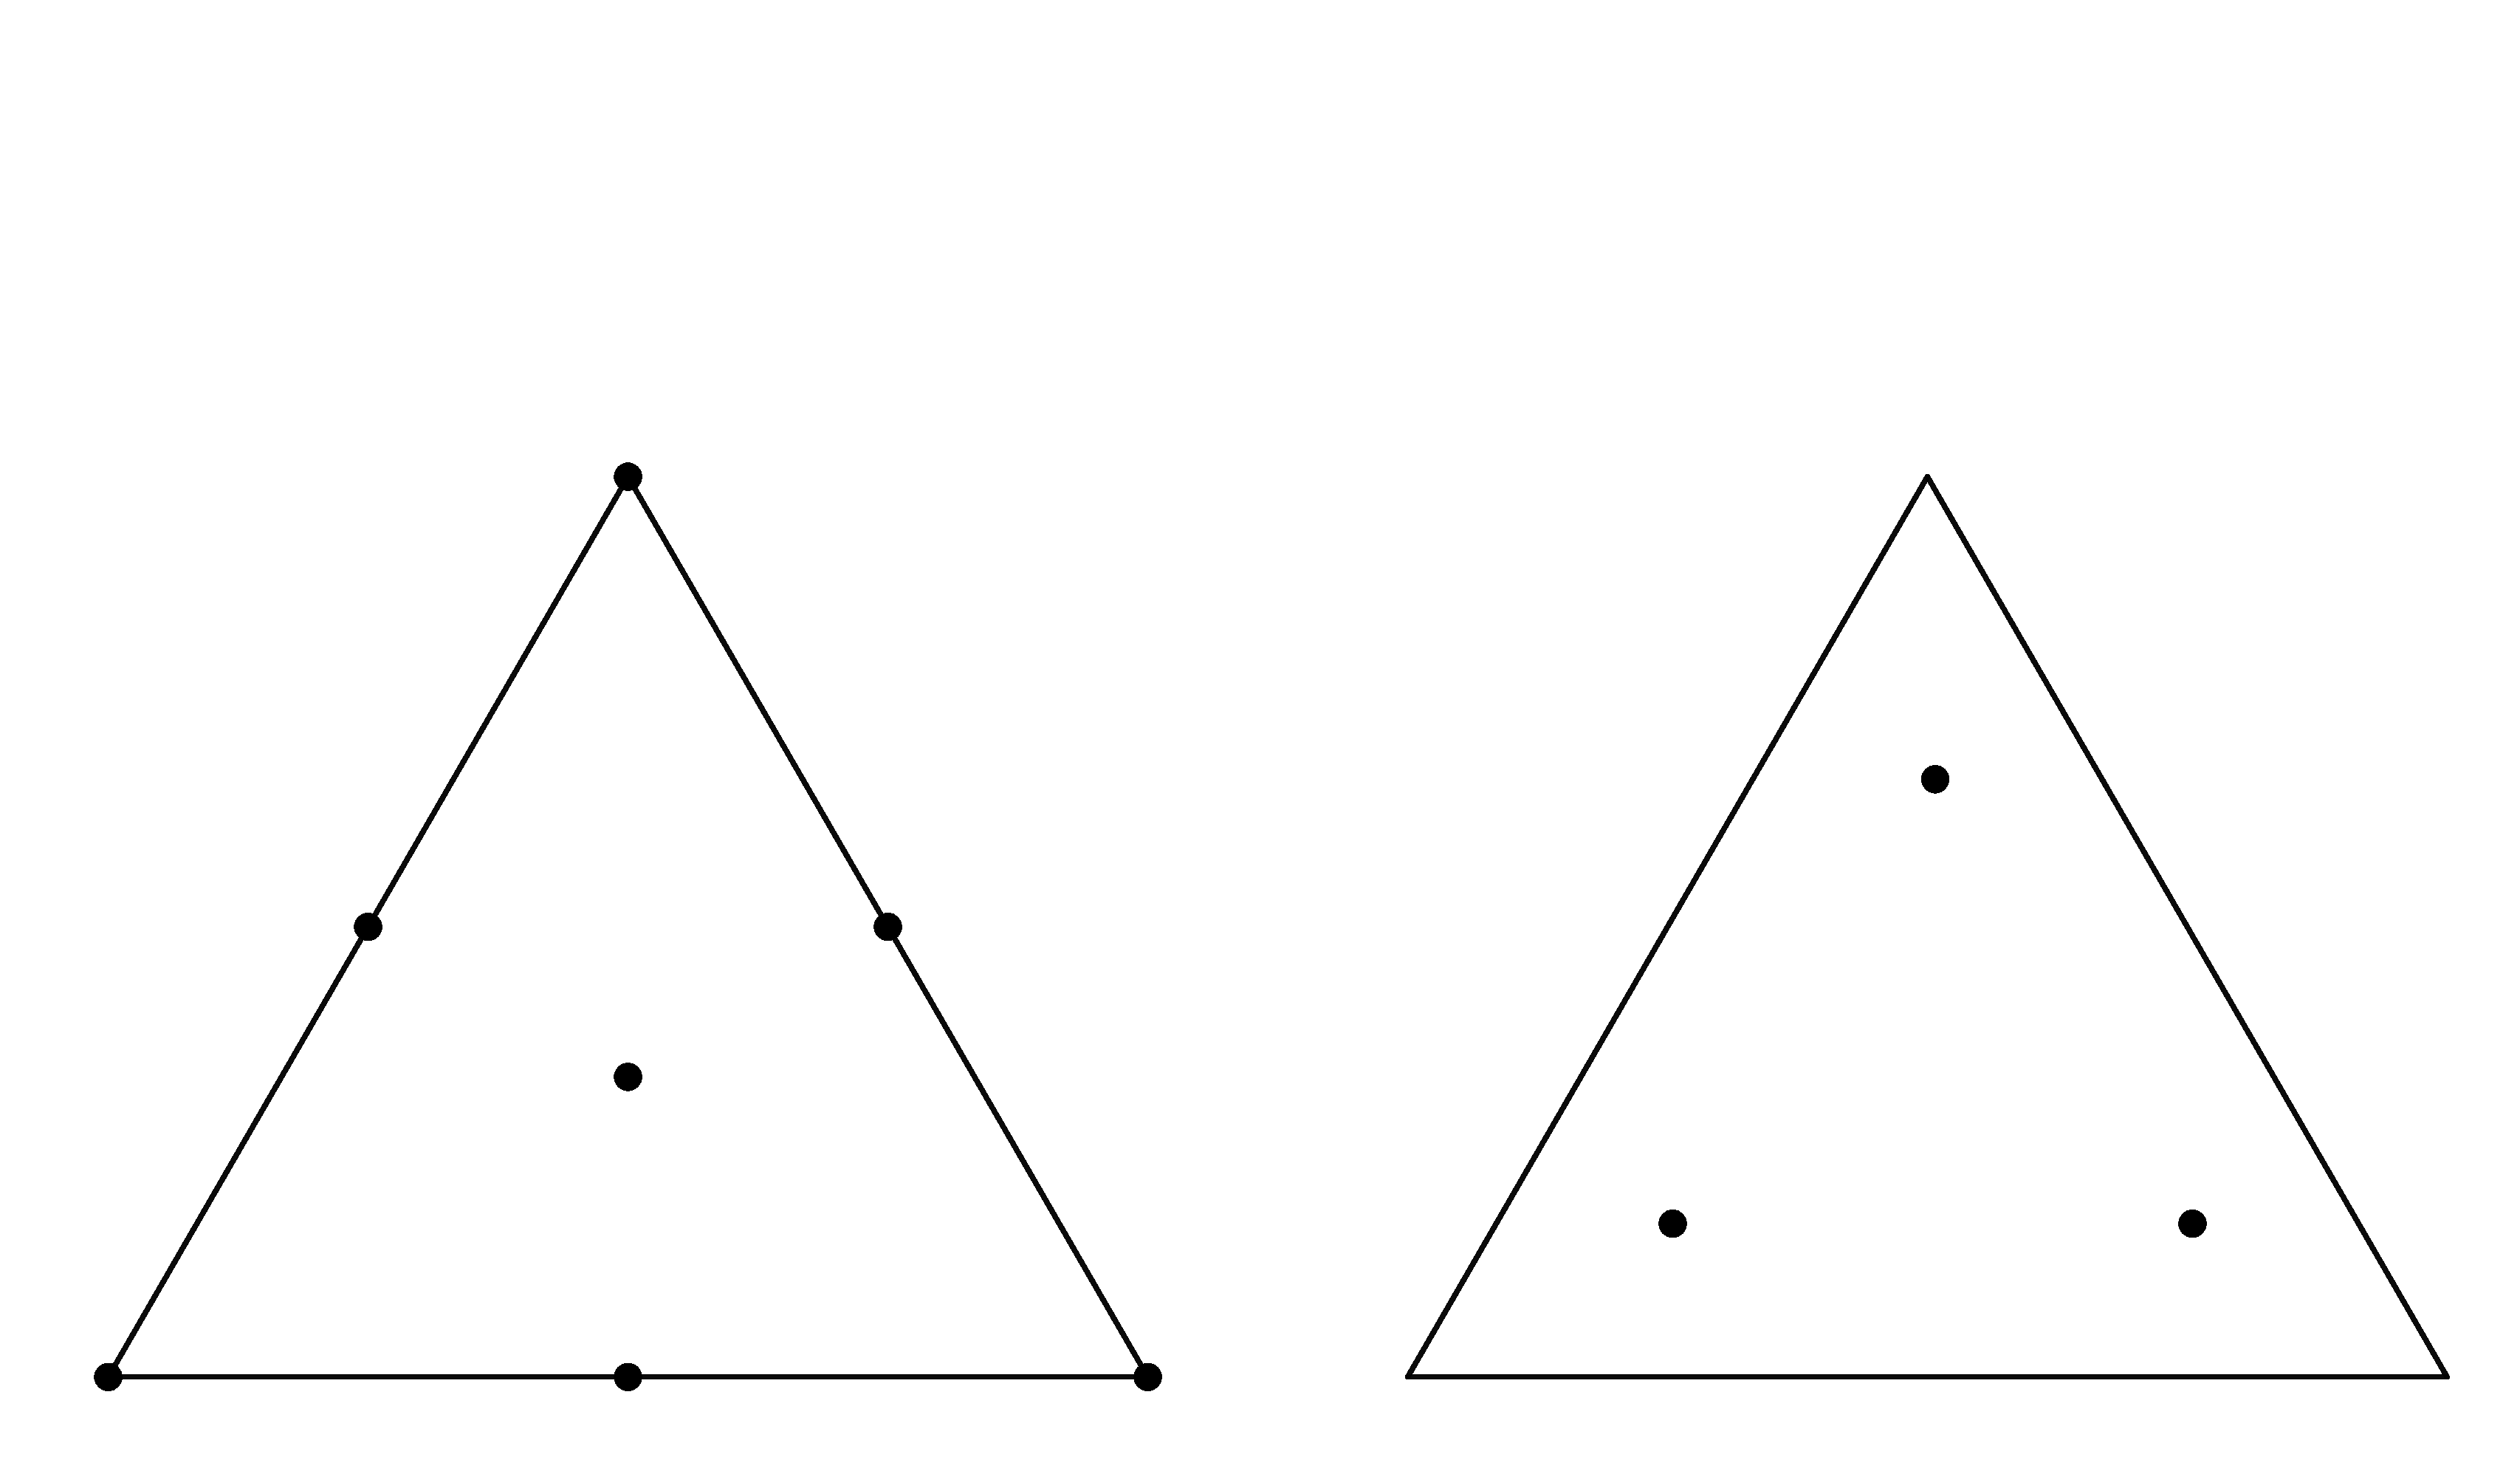
\includegraphics[trim=0cm 8cm 0cm 10cm, clip, width=15cm]{cr.pdf}
	\caption{Crouzeix-Raviart local DOFs for velocity and pressure.}
\end{figure}

Let $\{\Tau_h\}_h$ be a sequence of shape-regular and quasi-uniform meshes. Define $V_h$ and $Q_h$ as follows:

\begin{align}
    V_h &= \left\{ \Vector{v_h} \in H^1_0(\Omega): \Vector{v_h} \vert_T \in \left[ \PK{2}(T) \cup \Span{b_T} \right]^2 ~ \Forall T \in \Tau_h \right\}, \\
    Q_h &= \left\{ q_h \in \LT_0(\Omega): q_h \vert_T \in \PK{1}(T) ~ \Forall T \in \Tau_h \right\},
\end{align}

where $b_T \in \PK{3}(T)$ such that $b_T \vert_{\partial T} = 0$ and $b_T(\nu_T) = 1 ~ \Forall T \in \Tau_h$:

\subsection{Fortin operator}

Let $\tfortin: V \rightarrow V_h$ such that:

\begin{gather}
    \tfortin \Vector{v} \vert_T = \frac{1}{\theta_T} \left[ \int_T \diver \Vector{v} \begin{pmatrix}
        x - x_T \\
        y - y_T
    \end{pmatrix} \right] \Vector{b_T},
\end{gather}

we define the Fortin operator $\fortin: V \rightarrow V_h$ for the Crouzeix-Raviart element as follows:

\begin{gather}
    \fortin \Vector{v} = \fortinptpz \Vector{v} + \tfortin \left( \Vector{v} - \fortinptpz \Vector{v}\right),
\end{gather}

where $\fortinptpz$ is the Fortin operator for the $\PK{2}-\PK{0}$ element.

$\fortin$ satisfies the hypothesis of the \nameref{fortin} lemma, hence ensuring the discrete \textit{inf-sup} property for the Crouzeix-Raviart element.

\newpage
\subsection{Convergence}

We can formulate the following result:

\begin{proposition}
    Let $\{\Tau_h\}_h$ be a sequence of shape-regular and quasi-uniform meshes. Suppose $(\Vector{u}, p)$ is the solution of \eqref{weak_stokes}, and $(\Vector{u_h}, p_h)$ is the solution of \eqref{fem_stokes}. Then, we have that:

    \begin{gather}
        \lVert \Vector{u} - \Vector{u_h} \rVert_V + \lVert p - p_h \rVert_Q \lesssim \inf_{\Vector{v_h} \in V_h} \lVert \Vector{u} - \Vector{v_h} \rVert_V + \inf_{q_h \in Q_h} \lVert p - q_h \rVert_Q \lesssim h^2.
    \end{gather}
\end{proposition}

	\newpage
	\section{Tests}
	Now, the behavior of the $\LT$ and $\HO$ velocity errors, as well as the $\LT$ pressure error\footnote{Linear slope will be represented in \textcolor{solarized-green}{green}, quadratic slope in \textcolor{solarized-blue}{blue}, and cubic slope in \textcolor{solarized-yellow}{yellow}.}, on various meshes is being evaluated as the mesh size decreases, testing \ref{convergence}.


\subsection{Error trend}

\begin{figure}[!ht]
	\centering
	\includegraphics[width=15cm]{errorTrend.pdf}
	\caption{Error trend.}
\end{figure}

\newpage
\subsection{Bubbleless error trend}

\begin{figure}[!ht]
	\centering
	\includegraphics[width=15cm]{errorTrendNB.pdf}
	\caption{Bubbleless error trend.}
\end{figure}

\newpage
\subsection{Polynomial fits}

Here are the results for the polynomial fits. Given the relatively low pressure error on the initial mesh, an additional fit is performed solely on the tail. 

\lstinputlisting[caption=Polynomial fits.]{../results/errorTrend.txt}
\lstinputlisting[caption=Bubbleless polynomial fits.]{../results/errorTrendNB.txt}

\end{document}
